% main.tex — generated by paper-covert
% Venue: Remote Sensing of Environment (Elsevier)
% Source manuscript: output/manuscript/MANUSCRIPT_DRAFT.md (post paper-review-loop round 1)
% Readiness: PARTIAL -- interim checkpoint, gated on E8 (national multi-year run, in progress)
%            and PAPER_PLAN.md Section 24 Open Issue #8 (candidate-model adoption, unresolved)
% Engine: pdflatex + bibtex
%
% Do not edit this file directly; regenerate via /paper-covert.
% Fallback article class -- re-wrap with the real elsarticle class before final submission
% (see profiles/rse.yaml notes and SUBMISSION_MANIFEST.md).

\documentclass[11pt,a4paper]{article}

% preamble.tex — generated by paper-covert

\usepackage[utf8]{inputenc}
\usepackage[T1]{fontenc}
\usepackage{lmodern}
\usepackage[english]{babel}

% Math
\usepackage{amsmath, amssymb, amsthm}
\usepackage{mathtools}

% Tables and figures
\usepackage{graphicx}
\usepackage{booktabs}
\usepackage{tabularx}
\usepackage{longtable}
\usepackage{caption}
\usepackage{subcaption}
\usepackage{float}

% Bibliography (natbib + author-year, close to elsarticle-harv pending the real Elsevier class)
\usepackage{natbib}

% Cross-referencing
% (cleveref not used: the manuscript's internal "Section N.M" references are plain prose,
% not \ref-based, matching how the Markdown source was written -- see SUBMISSION_MANIFEST.md.)
\usepackage{hyperref}

% Page geometry
\usepackage[margin=1in]{geometry}

% URL handling in bibliography
\usepackage{url}

% Colour support for the pending/placeholder markers below.
% (No boxed "placeholder" environment is defined: this manuscript's [PENDING: E8] and
% [PLACEHOLDER ...] markers are inline bold/bracketed text in the source Markdown, not
% block-level content, so they render correctly as plain text -- no mdframed dependency
% needed, and mdframed.sty is not installed in this TeX Live 2018 environment.)
\usepackage{xcolor}

% Pending-revision figure tag
\newcommand{\figpending}{\textcolor{red!70!black}{\textbf{[FIGURE PENDING REVISION]}}}

% Citation placeholder used when a [CITE: ...] block survives conversion.
\newcommand{\citeplaceholder}[1]{\textcolor{red!70!black}{[CITE: #1]}}

% Pandoc's standard boilerplate command for compact (tight) itemize/enumerate lists.
\providecommand{\tightlist}{%
  \setlength{\itemsep}{0pt}\setlength{\parskip}{0pt}}

\hypersetup{
  colorlinks=true,
  linkcolor=blue!50!black,
  citecolor=blue!50!black,
  urlcolor=blue!50!black,
}

% metadata.tex — generated by paper-covert
% Title from PAPER_PLAN.md §21 Option 1 (the option used throughout the manuscript, see
% sections/00_title.md); author list intentionally left as a placeholder — this skill does
% not generate author information.

\title{A National, Polygon-Level Crop-Species Map of Australia from Sentinel-2: Presence-Gated Classification, Calibrated Yield, and Validation Against Official Statistics}

\author{[Author list and affiliations not yet supplied --- placeholder, per project convention: author information is never auto-generated.]}

\date{Draft of \today\ --- PARTIAL manuscript, interim checkpoint (see SUBMISSION\_MANIFEST.md)}

% Keywords (RSE requires 5-8; PAPER_PLAN.md does not pin a specific list, so these are
% drawn directly from the manuscript's own stated scope and methods, not invented content).
\newcommand{\keywordlist}{crop-type mapping; Sentinel-2; Segment Anything Model; presence detection; accuracy assessment; gradient boosting; Australia}


\begin{document}

\maketitle

\begin{center}
{\Large\bfseries A National, Polygon-Level Crop-Species Map of Australia from Sentinel-2: Presence-Gated Classification, Calibrated Yield, and Validation Against Official Statistics}

\vspace{0.5em}
[Author list and affiliations not yet supplied --- placeholder, per project convention: author information is never auto-generated.]
\end{center}

\vspace{1em}
\noindent\textit{\textbf{Interim checkpoint, not a submission-ready package.} This PDF was generated while the
national multi-year run (E8, 2017--2025) is still in progress (2 of 9 years complete) and while
PAPER\_PLAN.md \S24 Open Issue \#8 (whether to adopt a leading, not-yet-independently-reviewed
classifier candidate) remains unresolved. Every [PENDING: E8] marker in the source
manuscript is preserved below, unfilled. See SUBMISSION\_MANIFEST.md for the full
readiness statement.}

\vspace{1em}
\noindent\textbf{Keywords:} \keywordlist

% Generated by paper-covert from output/manuscript/sections_revised/01_abstract.md

\section*{Abstract}\label{abstract}

Australia's grains sector lacks a continent-wide, field-verified, paddock-scale crop-species map: existing global products classify cropland generically, and the closest Australian precedents are regional, not trained exclusively on field-verified ground truth. We present a national, polygon-level map that segments paddocks with the Segment Anything Model, classifies them into three groups (Canola, Cereal, Legume) with a gradient-boosted spectral-index classifier built from 2,194 field-verified Grains Research and Development Corporation (GRDC) National Variety Trial records, applies a presence gate to decide whether a segmented paddock is classified at all, and attributes a calibrated Cereal yield to classified paddocks. The completed 2024 national map contains 1,346,582 segmented polygons; 48.4\% carry a classification, and the remainder carry an explicit abstain reason rather than being silently dropped. Validated against independent Australian Bureau of Statistics (ABS) sown-area statistics across 133 censused Statistical Area Level 2 regions with no connection to the training pipeline, mapped canola composition tracks the official statistic closely (r = 0.82, median absolute error 5.5 percentage points --- below the 6.8\% floor set by ABS's own disagreement with a second official series), but the map over-calls crop-present area by 1.47-1.59x --- concentrated in Cereal and Legume, not Canola --- a presence-detection rather than classification problem, corroborated by independent comparison against WorldCereal and the National Land Use Map. A more theoretically principled phenology-shape presence gate closed the area-inflation gap in a regional test but disproportionately rejected real canola paddocks, and was rejected. We report this as a transferable caution for presence-gate design in crop mapping generally.

\subsection{Highlights}\label{highlights}

\begin{itemize}
\tightlist
\item
  National, field-verified, 10 m crop map of Australia: 1.35M paddocks, 3 classes.
\item
  Canola composition matches independent ABS statistics closely (r=0.82).
\item
  Map over-calls crop area 1.5x --- a presence, not classification, failure.
\item
  A more principled presence gate fixed area but broke canola recall; rejected.
\item
  Independent WorldCereal/NLUM comparison corroborates the presence diagnosis.
\end{itemize}

\subsection{Graphical Abstract}\label{graphical-abstract}

\emph{Reuses Fig. 1's elements: the six-stage pipeline schematic (Sentinel-2 time series $\rightarrow$ SAM
segmentation $\rightarrow$ paddock mask $\rightarrow$ spectral-index classifier $\rightarrow$ presence gate $\rightarrow$ Cereal yield
calibration) above a small real-output map panel, coloured by predicted class with
unclassified (abstained) paddocks shown in grey rather than omitted. See
\texttt{output/figures/Fig01\_hero.png} and its script \texttt{output/figures/scripts/Fig01\_hero.py}.}

% Generated by paper-covert from output/manuscript/sections_revised/02_introduction.md

\section{Introduction}\label{introduction}

Australia's grains sector --- wheat, barley, canola, and pulse/legume crops --- is a major export industry, yet no continent-wide, field-verified, species-resolved crop map exists at paddock scale. Official production and area statistics from the Australian Bureau of Statistics (ABS) and the Australian Bureau of Agricultural and Resource Economics and Sciences (ABARES) are available only at coarse administrative-region granularity, with no spatial detail below the Statistical Area Level 2 (SA2) or state level, and the two agencies disagree with each other by a median 6.8\% on national sown area --- an honest floor against which any finer-grained map should be judged, not a target of zero disagreement. A spatially explicit, species-resolved product would let growers, agronomists, and policy analysts see where each crop is actually grown, at the scale a single farm operates, rather than inferring it from a regional aggregate.

Remote sensing has made continent- and global-scale cropland mapping technically feasible, but scale and species resolution trade off against each other in practice. Products built for global coverage typically classify land as cropland versus non-cropland, or into a small number of broad crop-type groups defined by growing calendar rather than species, because building species-resolved training data at global scale is prohibitively expensive. Australia sits in a Southern Hemisphere, canola-and-legume-growing agricultural system that most global crop-calendar-based products were not designed around, so even where global coverage exists, its species resolution and seasonal assumptions may not transfer.

Three threads of prior work bear on this problem. Global crop-mapping infrastructure --- WorldCereal \citep{vantricht2023worldcereal}, foundation-model embeddings such as Presto \citep{tseng2024presto} and AlphaEarth \citep{brown2025alphaearth}, and generic land-cover products such as Esri/Impact Observatory's global land-use-land-cover layer \citep{karra2021esri} --- delivers broad coverage but coarse or generic crop-type resolution, and none has been evaluated for Australian species-level generalizability. Two Australian precedents come closer: an in-season Sentinel-2 classifier for six classes in Western Australia \citep{sharma2026wa} and a Sentinel-1/Sentinel-2/MODIS fusion classifier distinguishing cereals from canola in the Murray-Darling Basin \citep{alshammari2024mdb}. Both are regional rather than continent-wide, and both train on either another model's output or opportunistic harvester-derived labels rather than field-verified ground truth. A third thread addresses the paddock-boundary problem this map also depends on: CSIRO's ePaddocks/Graincast system \citep{lawes2022graincast} is the closest operational Australian precedent for boundary-plus-yield mapping at scale, while the Segment Anything Model (SAM; \citealp{kirillov2023sam}) --- the segmentation backbone used here --- and Fields of the World \citep{kerner2024fields}, a cloud-robust Sentinel-1/Sentinel-2 boundary-delineation benchmark that does not cover Australia, represent the general-purpose segmentation methods this paper draws on instead of a bespoke Australian boundary product.

The gap this leaves is specific: no published map combines continent-wide coverage, paddock-scale resolution, species-level (not merely cropland) classification, and training exclusively on field-verified ground truth, for the Australian grains system. Closing it exactly as originally scoped --- a full \textasciitilde10-species classifier trained via foundation-model fine-tuning --- proved not to be reachable at the field-verified label volume available: a 9-species classifier reached only macro F1 0.38, and fine-tuned Presto embeddings scored worse than hand-built spectral indices (macro F1 0.775 vs.~0.821) at this label volume. We report both as genuine negative results rather than silently narrowing scope without comment, and instead ship a 3-group classifier (Canola, Cereal, Legume) built on hand-engineered, day-of-year-binned spectral indices.

This paper makes two primary contributions. First, we present a national, polygon-level, three-class crop-species map of Australia at 10 m resolution, built end-to-end from open Sentinel-2 imagery and 2,194 field-verified GRDC National Variety Trial (NVT) records --- not another model's predictions or opportunistic harvester data. Every polygon carries a predicted class or an explicit abstain reason, a per-polygon confidence, and, for Cereal, a calibrated yield estimate; the map is validated against independent ABS sown-area statistics with no connection to the training pipeline. Second, we quantify and mechanistically explain a systematic area-inflation failure mode common to presence-only crop mapping --- the map over-calls crop-present area by 1.47-1.59x, concentrated almost entirely in the Cereal and Legume classes and essentially absent from Canola --- and report a negative result from the natural, more principled fix: a phenology-shape presence gate that closed the area-inflation gap but did so by disproportionately rejecting real canola paddocks, and was rejected for that reason. This is a transferable caution for presence-gate design in crop mapping generally, not only for this pipeline. Two further findings support these primary contributions rather than standing alone: a label-conflict resolution specific to point-based agronomic trial networks, where collapsing species to broad groups and hand-reviewing co-located trials measurably improves classifier performance; and a negative result for foundation-model embeddings against hand-built spectral indices at this label volume, reported above.

The remainder of this paper is organized as follows. Section 2 reviews related work in global crop mapping, Australian precedents, paddock-boundary delineation, and accuracy-assessment standards. Section 3 describes the study area and data sources. Section 4 details the segmentation, labelling, classification, presence-gating, and yield-calibration methodology. Section 5 reports classifier accuracy, the ABS validation, the phenology-gate experiment, yield calibration, and an independent spatial comparison against the WorldCereal and National Land Use Map (NLUM) products. Section 6 discusses the area-inflation finding and its implications for presence-gate design. Section 7 states limitations, including the map's largest current scope gap --- single-season (2024) national coverage, pending a planned multi-year national extension --- and Section 8 concludes.

% Generated by paper-covert from output/manuscript/sections_revised/03_related_work.md

\section{Related Work}\label{related-work}

\subsection{Global crop-mapping infrastructure and foundation models}\label{global-crop-mapping-infrastructure-and-foundation-models}

A growing ecosystem of global and continental crop-mapping products now provides open, regularly updated coverage. WorldCereal \citep{vantricht2023worldcereal} is the most directly comparable: a dynamic, open-source system producing seasonal maize, winter-cereal, and spring-cereal classifications and a general temporary-cropland extent layer from Sentinel-1 and Sentinel-2, tiled across 106 globally defined agro-ecological zones. It has no Canola or Legume class, reflecting its design priorities toward globally widespread cereal and maize systems rather than the Southern Hemisphere oilseed-and-pulse rotations that structure the Australian grains sector. Foundation-model embeddings have also been proposed as a general-purpose alternative to hand-engineered spectral features: Presto \citep{tseng2024presto} pretrains a lightweight transformer on multi-modal pixel time series (optical, radar, climate, terrain) for downstream fine-tuning, and AlphaEarth \citep{brown2025alphaearth} extends this idea to a general-purpose annual embedding at global scale. Generic land-use-land-cover products such as Esri/Impact Observatory's global layer \citep{karra2021esri} classify cropland as a single category without species or crop-type resolution at all.

This paper relates to this cluster as a local adaptation-and-comparison study with two genuine negative results rather than a novel infrastructure contribution. We fine-tuned Presto on our own field-verified labels and found it lost to hand-built, day-of-year-binned spectral indices (NDVI, a canola-specific flowering index, and a chlorophyll-fluorescence-related index) at this label volume and class granularity --- macro F1 0.775 versus 0.821 for the hand-built feature set, and markedly worse on canola detection specifically (74.2\% versus 89.0\% at a 5\% false-positive rate). Combining Presto embeddings with the hand-built features gave no improvement over the hand-built features alone (0.824 versus 0.821, within the noise of a size-matched control comparison). The most plausible cause is not that Presto's representation is unsuited to this problem, but that three of its nine expected input channel groups --- Sentinel-1 radar, ERA5 climate, and SRTM terrain --- are absent from our input data and must be passed as masked rather than genuinely observed; this is a data-availability limitation of our deployment, not necessarily a finding about Presto's architecture, and we report it as such. We also directly compared our national map against WorldCereal's 2021 products at the pixel level (Section 5.5): because WorldCereal has no Canola or Legume class, only the presence/absence extent layer and the wintercereals layer are checkable against our output, and both comparisons are reported with their full caveats rather than treated as ground truth.

\subsection{Australia-specific crop-type classification precedents}\label{australia-specific-crop-type-classification-precedents}

Two studies are the closest direct precedents. \citet{sharma2026wa} built an in-season Sentinel-2 classifier for six crop classes in Western Australia, using day-after-sowing-derived pseudo-labels for the bulk of training data supplemented by a smaller field-verified test set. \citet{alshammari2024mdb} fused Sentinel-1, Sentinel-2, and MODIS to distinguish cereals from canola across the Murray-Darling Basin, training on harvester-derived yield-map labels rather than recorded sowings. Both reach classification accuracies above 90\% within their respective study regions, and both represent substantial prior engineering effort. Neither, however, is continent-wide, and neither trains exclusively on field-verified ground truth: \citeauthor{sharma2026wa}'s pseudo-labels are model-derived, and \citeauthor{alshammari2024mdb}'s harvester labels are opportunistic records of what a combine harvested, not confirmed sowings. This paper's methodological position relative to both is to trade breadth of species resolution --- three broad groups rather than six specific crops --- for two things neither precedent has together: continent-wide coverage and training exclusively on GRDC National Variety Trial records, which are field-recorded sowings rather than another model's output or an opportunistic byproduct of harvest operations.

A third, operationally oriented precedent is CSIRO's Graincast system \citep{lawes2022graincast}, which combines a field-boundary product (ePaddocks) with a satellite-and-climate-driven yield model to monitor crop production across the Australian grainbelt at national scale. Graincast's boundary-plus-yield pattern is the closest operational analogue to what this paper attempts, and the original project brief for this work specified ePaddocks as the intended boundary source. In practice, this project replaced ePaddocks with Segment Anything Model (SAM)-based segmentation (Section 2.3) early in development; Graincast is cited here as the closest prior art for the general pattern, not as a method this paper builds on directly.

\subsection{Field and paddock boundary delineation}\label{field-and-paddock-boundary-delineation}

Paddock boundaries were delineated with the Segment Anything Model (SAM; \citealp{kirillov2023sam}), a general-purpose, promptable image-segmentation foundation model, applied here via the SAMGeo/PaddockTS geospatial wrapper with stock parameters. This is a departure from the project's original plan to use ePaddocks (Section 2.2) as the boundary source. Fields of the World \citep{kerner2024fields} is the most directly relevant methodological comparison point among purpose-built agricultural boundary-delineation methods: a cloud-robust Sentinel-1-and-Sentinel-2 field-boundary model evaluated against a multi-country benchmark. Its published benchmark does not include Australia, and its own documentation notes that only a model-predicted global product, not the curated benchmark itself, extends to the Australian continent; this absence of Australian ground-truth boundary data was itself a factor in the decision to use a general-purpose segmentation model rather than attempt to adapt a boundary-specific method without a local evaluation set.

\subsection{Accuracy-assessment standards for crop and land-cover maps}\label{accuracy-assessment-standards-for-crop-and-land-cover-maps}

\citet{olofsson2014goodpractices} set out the field's stated good-practice standard for map accuracy assessment and area estimation: stratified probability sampling of reference data, error matrices, and confidence intervals on both accuracy and estimated area. This standard is named here explicitly because it is \emph{not} what this paper's validation does, and the reason matters for how the results should be read. Olofsson-style area estimation requires a probability sample of reference labels stratified by map class; no such sample of field-verified crop-species labels exists for Australia at the density this would require, because the GRDC/NVT trial network is a purposively sited agronomic trial program, not a probability sample of the landscape. In its place, this paper validates against ABS sown-area statistics aggregated to the SA2 level --- an independent, non-training-derived, but itself uncertain reference (ABS and ABARES, its sister agency, disagree with each other by a median 6.8\% on national sown area) --- reporting composition and area-ratio comparisons rather than a stratified accuracy assessment with confidence intervals. We flag this explicitly as a methodological limitation (Section 7) rather than presenting the ABS comparison as if it satisfied the Olofsson-style standard.

\subsection{Positioning relative to the nearest competing approaches}\label{positioning-relative-to-the-nearest-competing-approaches}

The nearest competing approaches are, respectively, WorldCereal for global coverage without species resolution, and \citet{sharma2026wa} and \citet{alshammari2024mdb} for Australian species-level classification without continent-wide, exclusively field-verified training data. This paper's differentiation along the specific dimension of ground-truth provenance and geographic coverage --- continent-wide, three-class, trained end-to-end on field-recorded sowings --- is a genuine methodological edge purchased at the explicit cost of coarser species resolution than either Australian precedent and of not solving global species generalizability the way a foundation-model approach might eventually. We report this trade-off directly rather than only in retrospect: the original \textasciitilde10-species scope was not reachable at the available field-verified label volume (9-class macro F1 0.38), and the 3-group descoping is a finding about label-volume requirements for field-verified species classification, stated here in the Introduction and Methods rather than discovered by the reader only in the Results.

\emph{Note on data lineage}: \citet{newmanfurbank2021} describes the same underlying GRDC National Variety Trial network this paper's ground truth is drawn from. It is not an independent public dataset, and this paper does not point readers toward it as a substitute or independent replication source; it is cited here only to acknowledge the shared data lineage.

% Generated by paper-covert from output/manuscript/sections_revised/04_study_area_and_data.md

\section{Study Area and Data}\label{study-area-and-data}

\subsection{Study area}\label{study-area}

The completed national map covers continent-wide Australia, comprising 99,465 tiles (98.9\% of the national extent that National Land Use Map, NLUM, probability surfaces indicate carries meaningful agricultural probability for one of the three target crop groups) for the 2024 growing season. A 100 km $\times$ 100 km block in the Riverina region of New South Wales, a major mixed-cropping district, was used for an intensively validated nine-season (2017-2025) regional test of the identical pipeline, reported separately from the national result because only the regional extent currently has multi-year coverage (Section 3.2; Section 7, Limitation 1). Fig. 2 shows the national tile coverage, the Riverina regional block, and the SA2 regions used for validation (Section 3.3).

\begin{figure}[htbp]
\centering
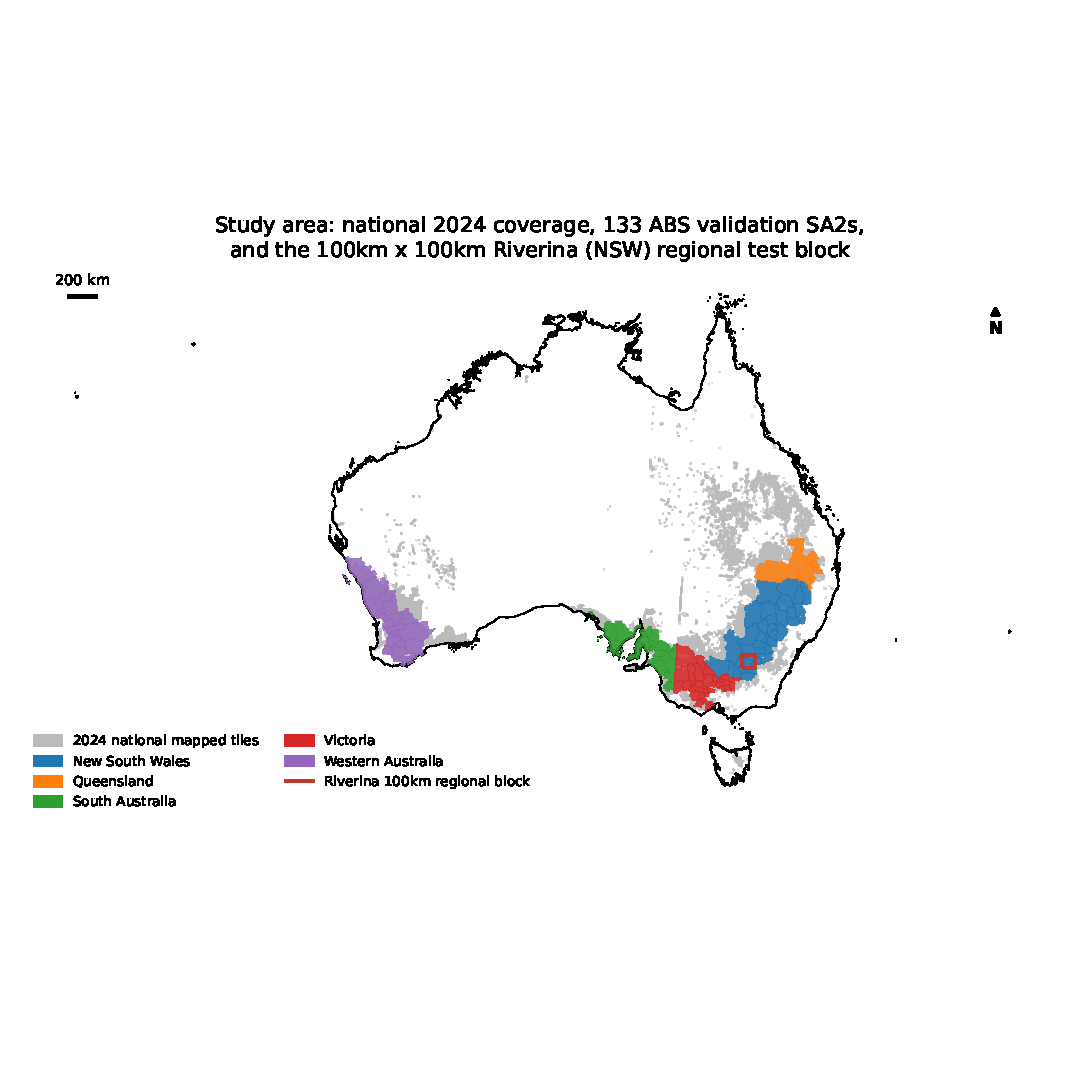
\includegraphics[width=0.85\textwidth]{figures/Fig02_study_area}
\caption{Study area. National extent of 2024 mapped tiles (grey; 99,465 tile centres), the 100km $\times$ 100km Riverina, NSW block used for the nine-year (2017-2025) regional test (red outline), and the SA2s used for ABS composition validation (coloured by state; EPSG:3577). 133 SA2s shown --- the $\geq$50\%-covered subset re-derived from the published per-SA2 cover table.}
\label{fig:2}
\end{figure}

\subsection{Temporal scope}\label{temporal-scope}

A single growing season, 2024, is complete and validated at national scale. Nine seasons (2017-2025) are complete at the 100 km regional scale. A national extension to the remaining eight seasons (2017-2023, 2025) is planned but has not yet been run at the time of this draft {[}PENDING: national 2017-2025 run, E8{]}; all results and figures in this paper that describe multi-year behaviour are explicitly regional, not national, and are reported as suggestive of but not proof of national multi-year generalization (Section 6.6).

\subsection{Data sources}\label{data-sources}

Table 1 summarizes the datasets used. Sentinel-2 surface-reflectance imagery was accessed via Digital Earth Australia's Analysis Ready Data product (\texttt{ga\_s2am/bm/cm\_ard\_3}) through the National Computational Infrastructure's datacube, at 10 m resolution, nationally, 2017-2025. Ground truth for training and validation is drawn from the Grains Research and Development Corporation (GRDC) National Variety Trial (NVT) network: field-verified, point-located records of sown crop per trial site, spanning 2017-2025 nationally. This dataset is covered by a data-use agreement and cannot be released or described at the site level (coordinates, trial identifiers, or yields); all reporting in this paper is aggregate. Independent validation uses ABS sown-area statistics, aggregated to the SA2 level, which have no connection to the training pipeline; ABARES production statistics provide a secondary cross-check on ABS itself, and the two agencies' median 6.8\% mutual disagreement on national sown area is the accuracy floor this paper measures its own map against (Section 5.2). NLUM v7 250 m per-commodity agricultural probability surfaces (2020-21) were used during national-scale inference to restrict segmentation and classification to tiles with non-trivial probability for one of the three target crop groups, and were separately used post hoc as an independent spatial-comparison product (Section 5.5); this is a different use of the same dataset and is described separately in each place it appears. Paddock boundaries were delineated with the Segment Anything Model (\texttt{vit\_h} checkpoint, stock parameters; \citealp{kirillov2023sam}) via the SAMGeo/PaddockTS wrapper; re-tuning SAM's segmentation parameters was investigated as a possible fix for a subset of poorly segmented polygons and ruled out as not cost-effective relative to the presence-gate and area-mask approach actually shipped.

\textbf{Table 1.} Dataset and pipeline summary.

\begin{longtable}[]{@{}
  >{\raggedright\arraybackslash}p{(\linewidth - 6\tabcolsep) * \real{0.2500}}
  >{\raggedright\arraybackslash}p{(\linewidth - 6\tabcolsep) * \real{0.2500}}
  >{\raggedright\arraybackslash}p{(\linewidth - 6\tabcolsep) * \real{0.2500}}
  >{\raggedright\arraybackslash}p{(\linewidth - 6\tabcolsep) * \real{0.2500}}@{}}
\toprule\noalign{}
\begin{minipage}[b]{\linewidth}\raggedright
Dataset
\end{minipage} & \begin{minipage}[b]{\linewidth}\raggedright
Role
\end{minipage} & \begin{minipage}[b]{\linewidth}\raggedright
Resolution / extent
\end{minipage} & \begin{minipage}[b]{\linewidth}\raggedright
Access
\end{minipage} \\
\midrule\noalign{}
\endhead
\bottomrule\noalign{}
\endlastfoot
Sentinel-2 (DEA ARD) & Primary imagery; day-of-year-binned spectral indices & 10 m, national, 2017-2025 & Open \\
GRDC / NVT trial records & Training and validation ground truth & Point-in-paddock, national, 2017-2025 & Data-use agreement; not releasable; aggregate reporting only \\
ABS sown-area statistics & Independent validation reference & SA2-level, 133 SA2s, national & Public \\
ABARES production statistics & Cross-check on ABS (6.8\% median mutual disagreement) & State / national & Public \\
NLUM v7 250 m Ag. Probability Surfaces & (a) National-run coverage mask; (b) independent spatial-comparison product & 250 m, national & Public \\
WorldCereal 2021 v100 & Independent spatial-comparison product & 10 m, national AU extent & Public (CC-BY 4.0) \\
Segment Anything Model (SAM) & Paddock-scale segmentation, stock parameters & 10 m-derived polygons & Open weights \\
\end{longtable}


\subsection{Preprocessing}\label{preprocessing}

Segmented polygons were retained only within a 5-300 ha area range with a compactness ratio (perimeter / sqrt(area)) of at most 8 --- a free, non-spectral presence signal derived purely from segmentation geometry, which retains 77.9\% of known crop paddocks in validation while rejecting 65\% of pasture polygons, at a cost of excluding 22\% of real crop paddocks that fall outside the size/shape mask. Fifty-one paddock-median spectral features were computed per retained polygon, binned by day-of-year across the growing season, from three indices: NDVI, a canola-specific flowering index following the general approach of \citet{ashourloo2019canola}, and a chlorophyll-fluorescence-related index. NVT trial points were matched to their enclosing SAM polygon; because 69.7\% of training trials share a segmented paddock with another NVT trial (31.8\% with a different crop, reflecting how trial networks co-locate multiple varieties), the original nine-species label scheme was collapsed to three broad groups, resolving 69\% of these label conflicts, and the remainder were resolved by hand review (Section 4.2).

\input{sections/05_methodology}
% Generated by paper-covert from output/manuscript/sections_revised/06_results.md

\section{Results}\label{results}

\subsection{Classifier accuracy}\label{classifier-accuracy}

The reviewed-and-cleaned label arm reached macro F1 0.821 under temporal transfer (training on trials sown 2022 or earlier, testing on 543 fixed trials sown 2023-2024) and 0.823 under spatial transfer (5-fold \texttt{GroupKFold} on trial site, scored on the same 543 fixed test trials); Table 2 and Fig. 3 report both confusion matrices and per-class precision/recall. Canola was detected at 89.0\% recall at a 5\% false-positive rate (average precision 0.944, ROC AUC 0.965) --- a stricter operating-point metric distinct from the standard-decision precision/recall in Table 2. Per-class F1 under temporal transfer was 0.90 (Cereal), 0.88 (Canola), and 0.69 (Legume); Legume is the floor in both splits (recall 73\% temporal, 70\% spatial), driven predominantly by Cereal paddocks being misclassified as Legume (23 of 279 true Cereal paddocks under temporal transfer, 22 of 279 under spatial transfer) rather than the reverse.

\begin{figure}[htbp]
\centering
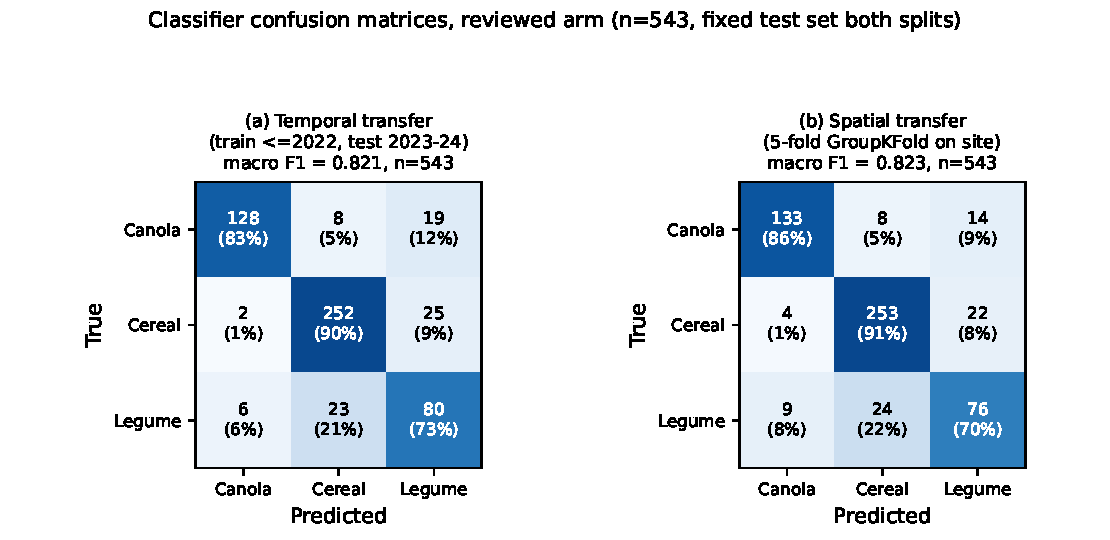
\includegraphics[width=0.85\textwidth]{figures/Fig03_confusion_matrices}
\caption{Classifier confusion matrices, ``reviewed'' arm, n=543 fixed test paddocks for both splits. (a) Temporal transfer (train $\leq$2022, test 2023-24): macro F1 0.821. (b) Spatial transfer (5-fold GroupKFold on site): macro F1 0.823. Legume is the floor in both splits (recall 73\% temporal, 70\% spatial), driven by Cereal leaking into Legume rather than the reverse.}
\label{fig:3}
\end{figure}

\textbf{Table 2.} Classifier accuracy by class and transfer split (reviewed-and-cleaned arm, 543 fixed test trials).

\begin{longtable}[]{@{}llllll@{}}
\toprule\noalign{}
Split (macro F1) & Class & Precision & Recall & F1 & n \\
\midrule\noalign{}
\endhead
\bottomrule\noalign{}
\endlastfoot
Temporal (0.821) & Canola & 0.94 & 0.83 & 0.88 & 155 \\
& Cereal & 0.89 & 0.90 & 0.90 & 279 \\
& Legume & 0.65 & 0.73 & 0.69 & 109 \\
Spatial (0.823) & Canola & 0.91 & 0.86 & 0.88 & 155 \\
& Cereal & 0.89 & 0.91 & 0.90 & 279 \\
& Legume & 0.68 & 0.70 & 0.69 & 109 \\
\end{longtable}


\subsection{National map and ABS validation: composition versus area}\label{national-map-and-abs-validation-composition-versus-area}

The completed 2024 national map contains 1,346,582 segmented polygons across 99,465 tiles (Table 1; Fig. 4). Of these, 48.4\% of polygons (34.4\% of total area) carry a classification; the remainder carry one of four explicit abstain reasons (\texttt{area\_below\_min}, \texttt{no\_crop\_signal}, \texttt{unsegmented\_blob}, \texttt{too\_few\_observations}) rather than being silently dropped. Validated against ABS sown-area statistics across the 133 SA2s where the mapped footprint covers at least 50\% of the SA2 (Section 4.6), mapped canola \emph{composition} --- its share of total mapped crop area --- tracks the ABS canola share closely: r = 0.82, median absolute error 5.5 percentage points, below the 6.8\% median disagreement between ABS and ABARES that this paper treats as the accuracy floor for any map-versus-official-statistic comparison (Section 3.3; Fig. 5a; Table 3).

\begin{figure}[htbp]
\centering
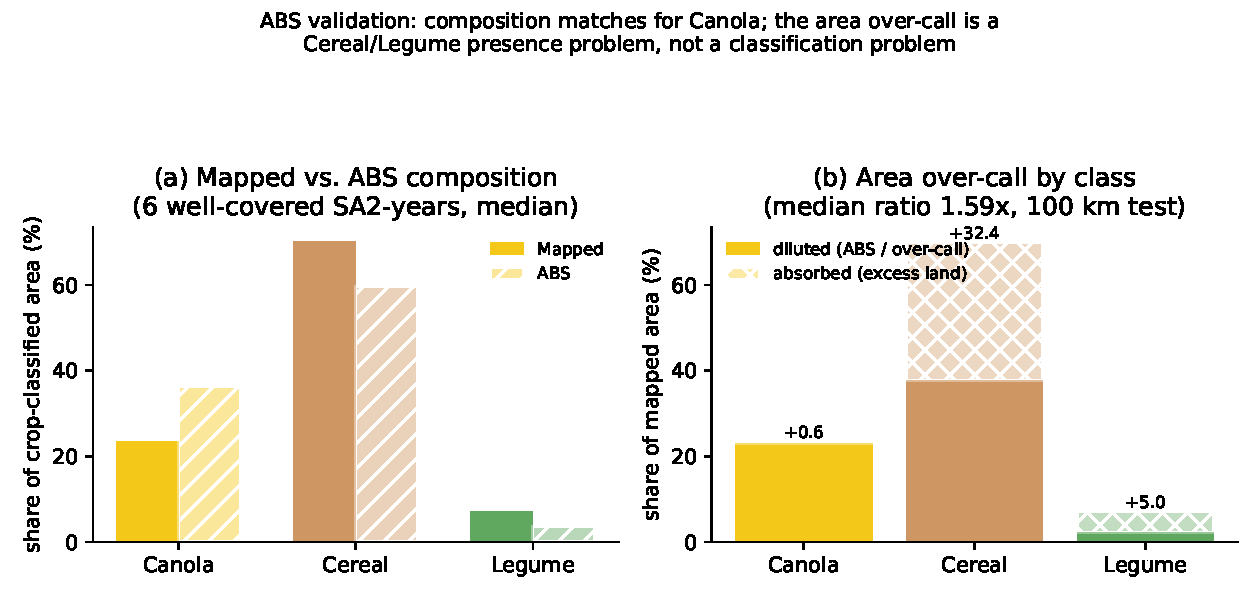
\includegraphics[width=0.85\textwidth]{figures/Fig05_abs_validation}
\caption{ABS validation: composition and area-inflation decomposition. (a) Mapped vs. ABS crop-share composition (Canola, Cereal, Legume), medians over the well-covered SA2-years. (b) Decomposition of the area over-call by class --- ABS share, the diluted share a perfect classifier would report given the measured over-call, and the absorbed excess --- showing the over-call sits almost entirely in Cereal and Legume, not Canola.}
\label{fig:5}
\end{figure}

\begin{figure}[htbp]
\centering
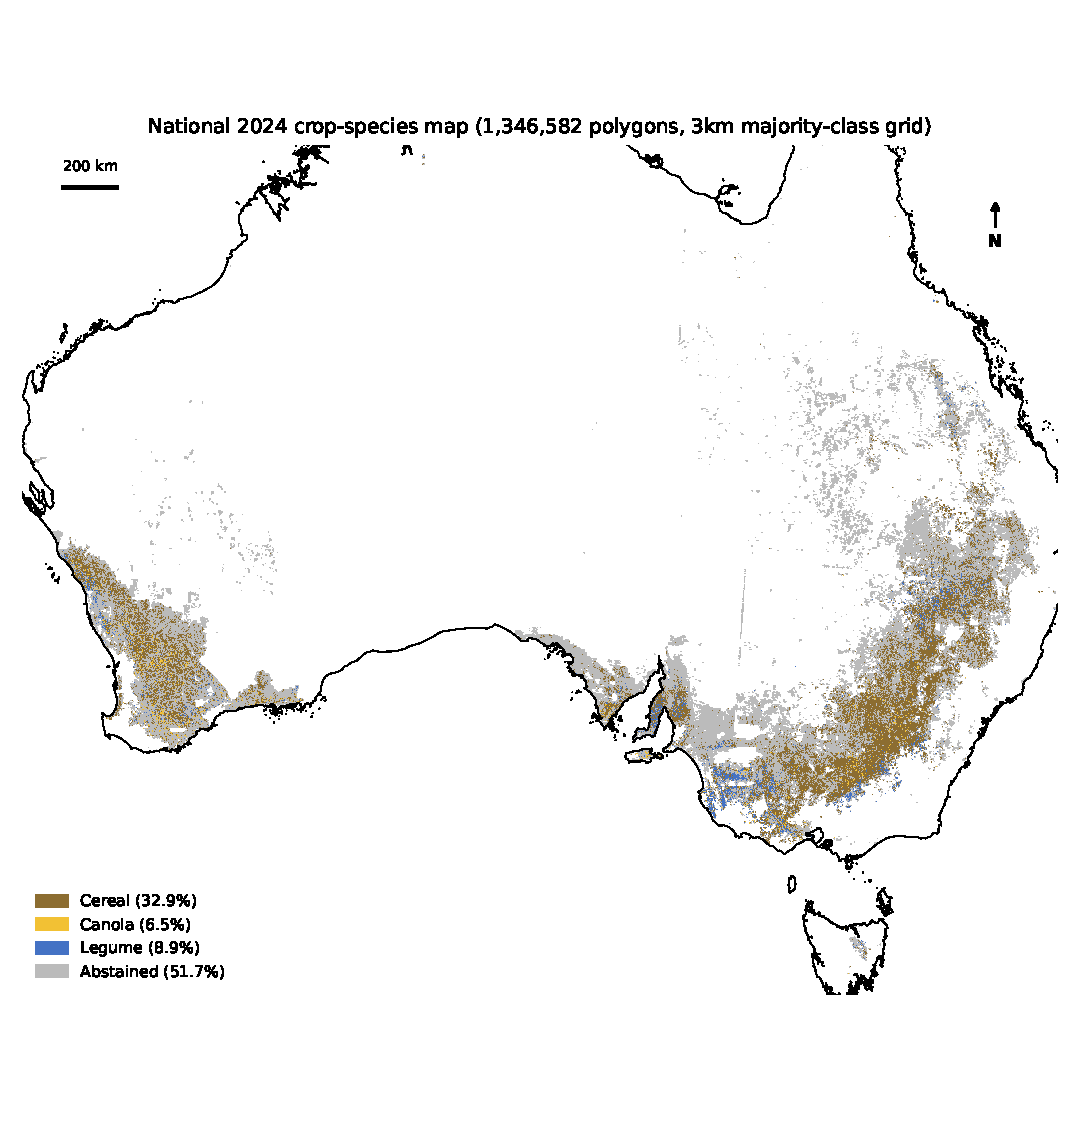
\includegraphics[width=0.85\textwidth]{figures/Fig04_national_map}
\caption{The national 2024 crop-species map. 1,346,582 segmented paddock polygons (EPSG:3577), rasterised to a 3km majority-class grid for legibility at national extent. Classified polygons coloured by predicted class: Cereal 32.9\% (443,008), Legume 8.9\% (119,578), Canola 6.5\% (88,180); unclassified polygons shown in grey (Abstained, 51.7\%, 695,816) rather than left blank, carrying one of four abstain reasons. Percentages are by polygon count, not by area.}
\label{fig:4}
\end{figure}

The map's absolute \emph{area}, however, over-calls crop-present land relative to ABS by 1.47x nationally and, independently, by 1.59x in the 100 km regional test --- the same mechanism reproduced at two spatial scales. Decomposing this over-call by class (Fig. 5b) shows it is concentrated almost entirely in Cereal (+23.2 percentage points of the over-called share) and Legume (+10.8 points), and is essentially absent from Canola (-0.3 points). Once the area over-call is divided out --- comparing the mapped canola share against the \emph{diluted} share a perfect classifier would report given the measured over-call, rather than against the raw ABS share directly --- canola composition matches almost exactly (13.1\% mapped versus a diluted expectation of 13.4\%). This is the central interpretive result of the paper: the map's dominant disagreement with official statistics is a presence-detection problem (calling too much land ``crop-present'' in the first place), not a crop-species classification problem, and it is reproduced independently at national and regional scale with the same class signature both times (Section 6.1).

\textbf{Table 3.} ABS validation summary, national scale, 133 SA2s. \texttt{diluted} is the crop-share ABS would imply if the area over-call were spread proportionally across classes; \texttt{absorbed} is the difference between that and the actual mapped share --- the excess this class's mapped area carries.

\begin{longtable}[]{@{}lllll@{}}
\toprule\noalign{}
Class & ABS share & Diluted share & Mapped share & Absorbed (points) \\
\midrule\noalign{}
\endhead
\bottomrule\noalign{}
\endlastfoot
Canola & 19.7\% & 13.4\% & 13.1\% & $-$0.3 \\
Cereal & 67.3\% & 45.8\% & 69.0\% & +23.2 \\
Legume & 8.7\% & 5.9\% & 16.7\% & +10.8 \\
\end{longtable}


Canola composition: r = 0.82, median absolute error 5.5 percentage points (n = 133). Area over-call: 1.47x national, 1.59x regional (100 km). ABS/ABARES mutual disagreement (the accuracy floor, Section 3.3): median 6.8\%.

\subsection{Legume classification error}\label{legume-classification-error}

A distinct, unresolved classification error sits on top of the presence-detection problem: Legume is mapped at 18.4\% of classified area nationally versus an ABS share of 8.7\%. An argmax-versus-mean-predicted-probability check (Section 4.6) rules out the cheap explanation that this is a decision-rule artefact (e.g., a systematic argmax tie-break) --- the two agree, so the disagreement reflects genuine classifier behaviour, not a threshold quirk. The mechanism remains open (Section 6.7, Section 7 Limitation 2); Section 5.1's confusion-matrix evidence (Cereal paddocks predicted as Legume more often than the reverse) is consistent with, but does not fully explain, the magnitude of the national over-prediction.

\subsection{Presence-gate experiment: a rejected fix}\label{presence-gate-experiment-a-rejected-fix}

A phenology-shape presence gate --- requiring both a green-up rise and a post-harvest senescence drop, rather than seasonal amplitude alone (Section 4.4) --- was tested against the full nine-year, 100 km regional dataset. On its own target metric, it succeeded: the regional area ratio against ABS fell from 1.59 to 1.00. But it did so at a real cost, visible only once presence recall is examined per crop rather than pooled: stacked presence recall (both the amplitude gate and the shape gate applied, as shipped) fell to 78.3\% for Canola, against 91.4\% for Cereal and 87.2\% for Legume --- the shape gate disproportionately rejects real canola paddocks specifically (Fig. 6; Table 4), even though canola recall under amplitude-only gating alone was 94.5\%, comparable to the other two crops. Because Canola is the class whose composition already matches ABS most closely (Section 5.2) and is this dataset's most reliably classified crop (Section 5.1), a gate that fixes the area-ratio number by disproportionately removing real canola paddocks trades a well-understood problem (area over-call, for which the map already ships a documented workaround; Section 6.4) for a worse, less legible one (silently dropping real canola detections). We therefore rejected the phenology-shape gate and shipped the simpler amplitude-only design, despite the shape gate's superior performance on the area-ratio metric alone (Section 6.2). A two-pass variant that exempts Canola from the shape gate restores canola recall to 94.5\% at no measured cost to Cereal or Legume recall, but has not been validated against the ABS area ratio and is reported as a future-work candidate, not a result (Section 7).

\begin{figure}[htbp]
\centering
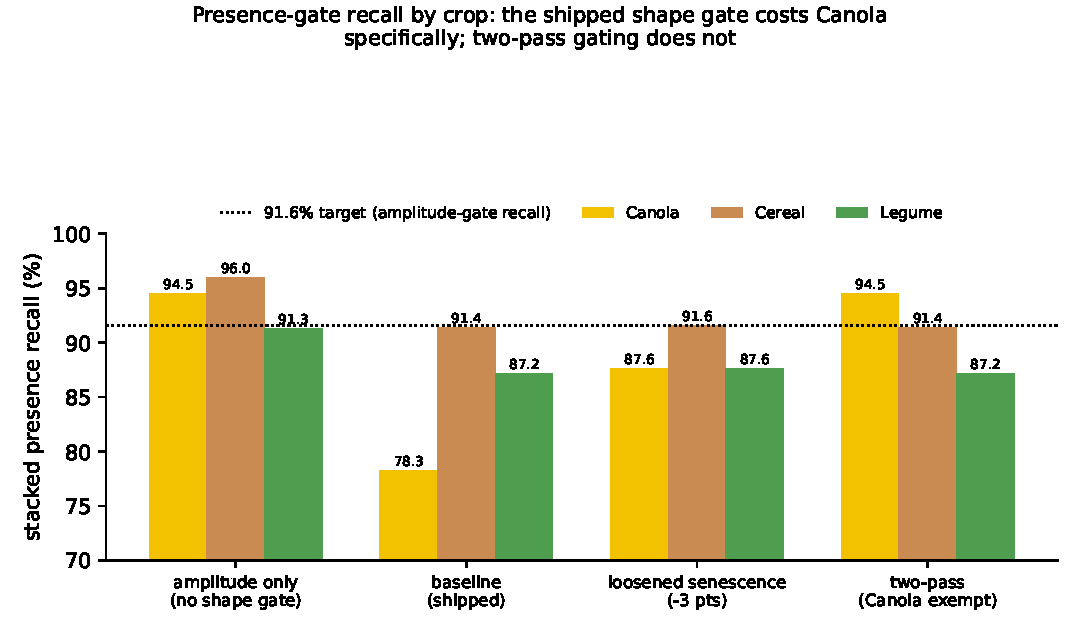
\includegraphics[width=0.85\textwidth]{figures/Fig06_gate_tradeoff}
\caption{Presence-gate trade-off. Stacked presence recall (amplitude gate AND presence-shape gate both applied) by crop, across four gate configurations. The shipped (baseline) configuration trades Canola recall (94.5\%$\rightarrow$78.3\%) for no change in Cereal/Legume recall relative to amplitude-only; two-pass gating (Canola exempted from the shape gate) restores Canola to 94.5\% at no cost to the other classes but is not yet validated against the ABS area ratio.}
\label{fig:6}
\end{figure}

\textbf{Table 4.} Presence recall by crop for three tested phenology-shape gate configurations, each stacked with the amplitude gate (100 km regional dataset). None of these three is the design actually shipped to production, which applies the amplitude gate alone (94.5\% Canola recall on this population, Section 4.4) and was retained because the phenology-shape gate's area-ratio gain came at the Canola-recall cost shown below.

\begin{longtable}[]{@{}
  >{\raggedright\arraybackslash}p{(\linewidth - 8\tabcolsep) * \real{0.2000}}
  >{\raggedright\arraybackslash}p{(\linewidth - 8\tabcolsep) * \real{0.2000}}
  >{\raggedright\arraybackslash}p{(\linewidth - 8\tabcolsep) * \real{0.2000}}
  >{\raggedright\arraybackslash}p{(\linewidth - 8\tabcolsep) * \real{0.2000}}
  >{\raggedright\arraybackslash}p{(\linewidth - 8\tabcolsep) * \real{0.2000}}@{}}
\toprule\noalign{}
\begin{minipage}[b]{\linewidth}\raggedright
Gate configuration
\end{minipage} & \begin{minipage}[b]{\linewidth}\raggedright
Pooled recall
\end{minipage} & \begin{minipage}[b]{\linewidth}\raggedright
Canola
\end{minipage} & \begin{minipage}[b]{\linewidth}\raggedright
Cereal
\end{minipage} & \begin{minipage}[b]{\linewidth}\raggedright
Legume
\end{minipage} \\
\midrule\noalign{}
\endhead
\bottomrule\noalign{}
\endlastfoot
Phenology-shape, baseline threshold & 87.0\% & 78.3\% & 91.4\% & 87.2\% \\
Phenology-shape, loosened senescence ($-$3 pts) & 89.6\% & 87.6\% & 91.6\% & 87.6\% \\
Phenology-shape, two-pass (Canola exempt) & 91.3\% & 94.5\% & 91.4\% & 87.2\% \\
\end{longtable}


\subsection{Independent spatial comparison: WorldCereal and NLUM}\label{independent-spatial-comparison-worldcereal-and-nlum}

Because both the ABS validation (Section 5.2) and the Legume classification check (Section 5.3) rely on the same broad type of reference data (official area/production statistics) as each other, we additionally compared the national map spatially, at the pixel level, against two products with no connection to this project's own pipeline: WorldCereal 2021 v100 and NLUM v7 250 m per-commodity probability surfaces, on a stratified sample of 250,000 national paddock centroids (Section 4.6). Both comparisons carry a three-year reference-year mismatch (2021 versus this map's 2024) and are reported with that caveat throughout.

Against WorldCereal's \texttt{temporarycrops} layer, our classified-versus-abstained presence call agrees at 73.1\% overall, and the agreement is symmetric: 73.0\% of our abstained points are also called ``no-crop'' by WorldCereal, and 73.2\% of our classified points are also called ``crop.'' Against WorldCereal's \texttt{wintercereals} layer, agreement on the Cereal class specifically is markedly weaker --- 49.6\% of the points our map calls Cereal are also called \texttt{wintercereals}-positive by WorldCereal --- a real disagreement, not sampling noise at this sample size (n=82,411), though WorldCereal is an independent product rather than ground truth and this disagreement does not by itself establish which product is correct.

NLUM's per-commodity probability surfaces, which unlike WorldCereal cover all three of our target groups directly, show a consistent enrichment pattern: median NLUM oilseed probability at our Canola-classified points is 6.4 times the median at our abstained points (the largest ratio in its column, correctly identifying Canola as the class most enriched for oilseed probability), and median legume probability at our Legume-classified points is 1.6 times the abstained-point median (likewise the largest ratio in its column). Independently of the classification comparison, NLUM's grazing-probability layer corroborates the presence-gate mechanism from an unrelated data source: median grazing probability is 33.8\% at our abstained points versus 10.8\% at our classified points, consistent with this project's earlier finding, from a retired absence-labelled grazing dataset (Section 6.4), that abstained land preferentially overlaps land NLUM independently rates as probable grazing country rather than being a uniform sample of ``everything the classifier could not decide about.''

\subsection{Multi-year regional evidence}\label{multi-year-regional-evidence}

Across the nine-year (2017-2025), 100 km regional re-run, classified share ranged from 52.5\% (2018) and 59.0\% (2017) up to 78.5\% (2025); mean NDVI amplitude was correspondingly lowest in 2018 (0.42) and 2017 (0.46) against 0.60-0.62 in 2024-2025 (Fig. 7a). We attribute the two weak years to Sentinel-2B's mid-2017 operational start (reducing revisit frequency and cloud-gap robustness in the earliest seasons) and a documented drought in 2018 respectively (Section 6.6). Polygon geometric stability across the same nine years --- independent of any spectral classification --- peaked in the 25-100 ha range (the range real paddocks predominantly occupy) and fell at both smaller and larger extremes, an independent, purely geometric corroboration of the area/compactness presence mask (Section 4.1). This regional evidence is suggestive of, but does not establish, similar behaviour at national scale; Figure 7's national panel and the corresponding national multi-year totals are explicitly reserved and left blank pending the national multi-year extension \textbf{{[}PENDING: national 2017-2025 run, E8{]}}.

\begin{figure}[htbp]
\centering
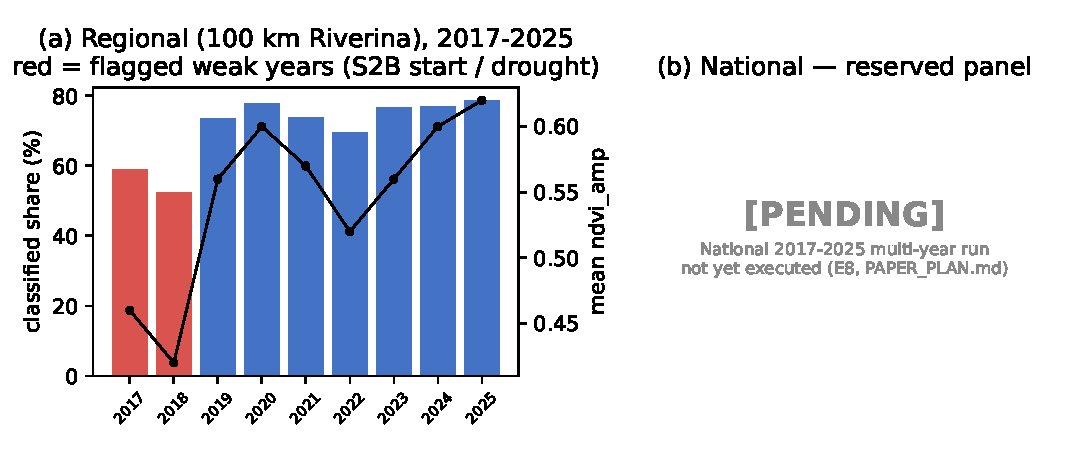
\includegraphics[width=0.85\textwidth]{figures/Fig07_multiyear_regional}
\caption{Multi-year regional evidence, with a reserved national panel. (a) Year-by-year classified share and mean \texttt{ndvi\_amp}, 2017-2025, 100km Riverina box; 2017 and 2018 (red) are flagged as structurally weaker years, attributed to Sentinel-2B's mid-year operational start and a genuine drought respectively. (b) \textbf{[PENDING: E8]} --- the equivalent national series is reserved but intentionally left blank pending the national 2017-2025 multi-year run; do not read panel (b) as a null result.}
\label{fig:7}
\end{figure}

\subsection{Cereal yield}\label{cereal-yield}

The Cereal yield model reached a spatial-transfer root-mean-square error of 1.21 t/ha (30.4\% of the 3.97 t/ha median observed yield). The ABS calibration factor (0.6248, fit on one year of ABS data) checked to within +3.1\% to +18.1\% of ABS-implied yield on two held-out years (Fig. 8; Table 5). Both raw (NVT-trial-equivalent) and ABS-calibrated yield columns are shipped on every classified Cereal polygon (Section 4.5).

\begin{figure}[htbp]
\centering
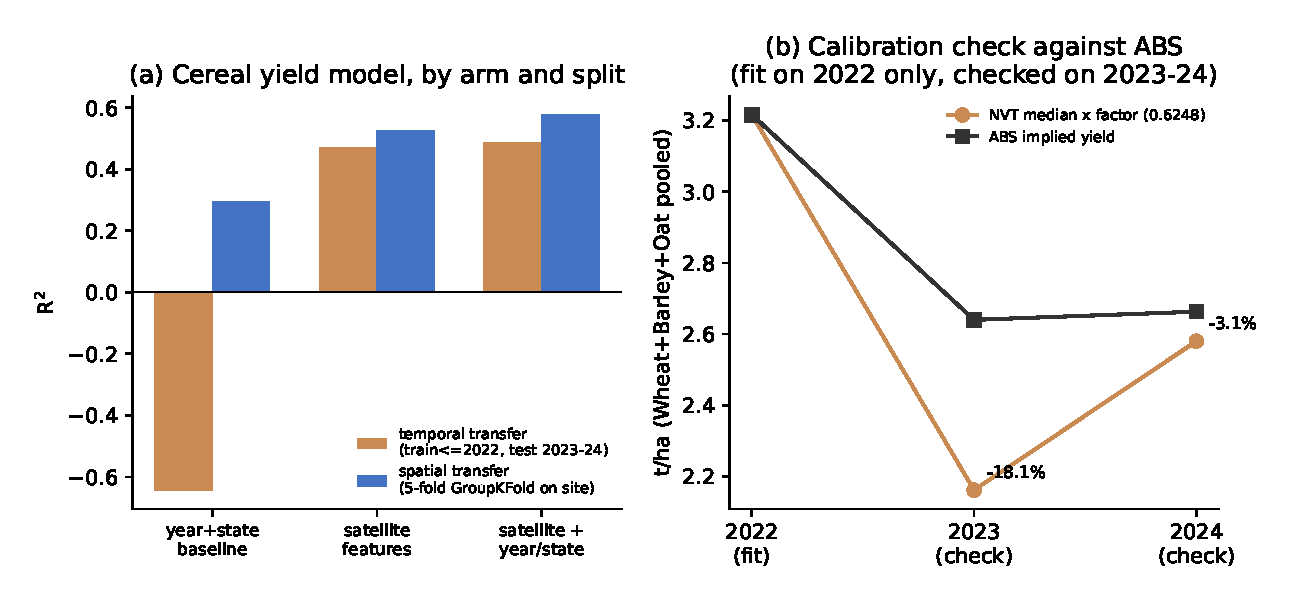
\includegraphics[width=0.85\textwidth]{figures/Fig08_yield_summary}
\caption{Cereal yield model performance and ABS calibration. Aggregate-only by design --- no per-trial predicted-vs-actual scatter is shown, since each point would be a single NVT trial record covered by the GRDC NDA. (a) R\textsuperscript{2} by model arm (year+state baseline, satellite features, satellite+year/state) under temporal transfer (train $\leq$2022, test 2023-24) and spatial transfer (5-fold GroupKFold on site). (b) Calibration check: NVT-median-factor (0.6248) calibrated yield vs. ABS-implied yield, fit on 2022 only and checked on 2023-24 (+3.1\% / +18.1\% error).}
\label{fig:8}
\end{figure}

\textbf{Table 5.} Cereal yield model performance (pooled Wheat/Barley/Oat, satellite-index features), before ABS calibration.

\begin{longtable}[]{@{}
  >{\raggedright\arraybackslash}p{(\linewidth - 8\tabcolsep) * \real{0.2000}}
  >{\raggedright\arraybackslash}p{(\linewidth - 8\tabcolsep) * \real{0.2000}}
  >{\raggedright\arraybackslash}p{(\linewidth - 8\tabcolsep) * \real{0.2000}}
  >{\raggedright\arraybackslash}p{(\linewidth - 8\tabcolsep) * \real{0.2000}}
  >{\raggedright\arraybackslash}p{(\linewidth - 8\tabcolsep) * \real{0.2000}}@{}}
\toprule\noalign{}
\begin{minipage}[b]{\linewidth}\raggedright
Split
\end{minipage} & \begin{minipage}[b]{\linewidth}\raggedright
Arm
\end{minipage} & \begin{minipage}[b]{\linewidth}\raggedright
n
\end{minipage} & \begin{minipage}[b]{\linewidth}\raggedright
R\textsuperscript{2}
\end{minipage} & \begin{minipage}[b]{\linewidth}\raggedright
RMSE (t/ha)
\end{minipage} \\
\midrule\noalign{}
\endhead
\bottomrule\noalign{}
\endlastfoot
Temporal (train $\leq$2022, test 2023-24) & Year+state baseline & 279 & $-$0.643 & 2.111 \\
& Satellite features & 279 & 0.471 & 1.197 \\
& Satellite + year/state & 279 & 0.486 & 1.181 \\
Spatial (5-fold GroupKFold on site) & Year+state baseline & 1,119 & 0.294 & 1.473 \\
& Satellite features & 1,119 & 0.526 & 1.207 \\
& Satellite + year/state & 1,119 & 0.577 & 1.140 \\
\end{longtable}


ABS calibration factor: 0.6248 (fit on one year), checked +3.1\% to +18.1\% against ABS-implied yield on two held-out years. Canola yield is not shipped: an optical-only model's coefficient of determination (0.27) did not exceed a trivial year-and-state-mean baseline (0.29), and no yield estimate is shipped for a class where the model does not outperform simply guessing the season and region (Section 7, Limitation 5).

\textbf{{[}PENDING --- depends on E8, not fabricated here{]}}: national multi-year (2017-2025) polygon and area totals by year (Table 6); national year-over-year canola/cereal/legume share trends; any claim that the single-national-season (2024) results reported above generalize nationally across seasons --- the regional nine-year evidence in Section 5.6 is suggestive, not proof, at national scale.

% Generated by paper-covert from output/manuscript/sections_revised/07_discussion.md

\section{Discussion}\label{discussion}

\subsection{A presence-detection failure, not a classification failure}\label{a-presence-detection-failure-not-a-classification-failure}

The central interpretive result of this paper is that the map's dominant disagreement with independent ABS statistics is a presence-detection problem rather than a species-classification problem. Three independent lines of evidence converge on this reading. First, canola \emph{composition} matches ABS closely (r=0.82) while total mapped \emph{area} over-calls ABS by 1.47-1.59x, and dividing out the over-call recovers near-exact canola-share agreement (Section 5.2) --- the kind of pattern a presence problem produces (too much land called ``crop-present,'' with the crop mix among that land roughly right) rather than a classification problem (the right amount of land called crop, with the wrong species assigned to some of it). Second, the same over-call magnitude and the same class concentration (Cereal and Legume, not Canola) reproduce independently at national and 100 km-regional scale, which a spurious artefact of one particular region or one particular year would not do. Third, the independent WorldCereal and NLUM spatial comparisons (Section 5.5), built from entirely separate data and with no connection to the ABS validation, corroborate the same diagnosis from a different angle: presence agreement against WorldCereal is symmetric and moderate (73\% both directions) rather than one-sidedly poor, and NLUM's independent grazing-probability layer shows abstained land is systematically more grazing-like than classified land --- consistent with genuine non-cropped land being the dominant source of the abstained population, rather than the classifier failing to recognize crops it should have recognized.

\subsection{The phenology-gate result as a general caution}\label{the-phenology-gate-result-as-a-general-caution}

The phenology-shape presence gate (Section 5.4) is, on paper, the more principled fix: it requires the shape evidence a real crop's growing season should produce (green-up, then senescence) rather than treating any sufficiently large seasonal amplitude as evidence of cropping. It also worked, on its own target metric --- the regional area ratio fell from 1.59 to 1.00, essentially eliminating the area-inflation problem this paper otherwise reports as its most consequential limitation. We rejected it anyway, because the metric it was evaluated against first (area ratio) was not the metric that mattered most for the map's usefulness (per-crop presence recall), and only checking recall per crop, not pooled, revealed that the fix worked by disproportionately removing real canola paddocks --- the map's best-classified and most ABS-consistent crop. We report this as a transferable methodological caution for presence-gate design in crop mapping generally, independent of this specific pipeline: a fix that is more theoretically principled, and that succeeds on its own headline target metric, can still be the wrong choice to ship, if evaluating it on a single pooled metric conceals which sub-population absorbs the improvement's cost. The appropriate response to a design choice like this is not to assume the more sophisticated option is better because it is more sophisticated, but to evaluate it on the metric that actually matters for the map's use, broken out by the sub-populations a pooled metric can hide.

\subsection{Foundation-model embeddings did not help here}\label{foundation-model-embeddings-did-not-help-here}

The Presto negative result (Section 5.1, Section 2.1) is worth discussing on its own terms rather than only as a methods footnote, because it runs against a common framing in the current crop-mapping literature that foundation-model embeddings straightforwardly outperform hand-engineered features. At this label volume (2,194 field-verified trials) and this class granularity (three broad groups), they did not: Presto alone underperformed hand-built spectral indices, and combining the two gave no measurable improvement over the hand-built features alone. We do not read this as evidence that Presto's architecture is unsuited to crop mapping in general --- three of its nine expected input channel groups (Sentinel-1 radar, ERA5 climate, SRTM terrain) were unavailable in this deployment and had to be passed as masked rather than genuinely observed, a specific, testable, and plausible explanation for the gap that this paper's data availability did not allow us to close. The result is reported as a data point against unconditional ``foundation models win'' claims in this literature, conditioned explicitly on label volume, class granularity, and input-channel completeness, not as a general verdict on foundation-model embeddings for crop mapping.

\subsection{The abstain-reason and confidence design as the map's actual answer to area inflation}\label{the-abstain-reason-and-confidence-design-as-the-maps-actual-answer-to-area-inflation}

Because every polygon in the national map carries either a predicted class or one of four explicit abstain reasons, plus a per-polygon NDVI-amplitude value and classification confidence, a downstream user who needs area-accurate rather than composition-accurate output already has the information required to filter toward a tighter, more conservative view of the map without waiting for a future methodological fix. This design choice was itself informed by an earlier failure: an initial design considered building an explicit absence-labelled ``non-crop'' class from presence-only farmer-recorded grazing records, and abandoned it after finding that 78.5\% of a deliberately hard stratum of grazing paddocks passed the same crop-presence test as known crop paddocks --- the negative labels themselves were not reliably negative, because presence-only farmer records cannot straightforwardly be inverted into confirmed absence labels. The abstain-reason and confidence fields shipped instead are the map's considered response to that failure mode: rather than force a binary crop/non-crop decision the available negative-label data could not support reliably, the map reports its uncertainty explicitly, on every polygon, as a first-class output field rather than a caveat buried in accompanying documentation.

\subsection{A covariate's value is task-dependent, not pipeline-dependent}\label{a-covariates-value-is-task-dependent-not-pipeline-dependent}

Two further findings, obtained after the results above were first drafted, add a second general caution alongside the phenology-gate result (Section 6.2). Sentinel-1 was re-tested against the current best classifier candidate --- the shipped model's three indices plus six band-derived indices from \citet{sharma2026wa}, an internally tested but not-yet-adopted feature set discussed further in Section 7 --- rather than the retired three-index baseline against which it was originally measured (Section 5.4, Section 6.3). Against this stronger baseline, Sentinel-1 regresses classifier accuracy by 0.023 macro F1 (temporal) and 0.018 (spatial), concentrated specifically on the Legume class (F1 0.82 to 0.77) --- the same class Sentinel-1 originally appeared to help. Permutation importance explains the reversal mechanistically: the Sharma et al.~red-edge index already resolves most of the Legume/Cereal confusion Sentinel-1 previously corrected (importance +0.134 without Sentinel-1), and once that confusion is resolved, Sentinel-1's additional feature columns have little signal left to contribute and instead dilute the model on a training set that did not grow to match them (importance collapsing to +0.018, with every other feature family scoring negative). The same evaluation against the model actually shipped for Cereal yield produces the opposite result: Sentinel-1 clearly improves yield prediction, adding 0.092 R\textsuperscript{2} on the yield model's own operational (satellite-plus-year/state, temporal-transfer) bar --- its largest gain in any arm tested. A parallel reversal runs the other way: the same band-derived indices that improve classification regress canola yield prediction when substituted for the shipped model's three simpler indices, with temporal R\textsuperscript{2} falling from 0.206 to 0.012. Table 7 summarizes all three results together.

\begin{longtable}[]{@{}
  >{\raggedright\arraybackslash}p{(\linewidth - 8\tabcolsep) * \real{0.2000}}
  >{\raggedright\arraybackslash}p{(\linewidth - 8\tabcolsep) * \real{0.2000}}
  >{\raggedright\arraybackslash}p{(\linewidth - 8\tabcolsep) * \real{0.2000}}
  >{\raggedright\arraybackslash}p{(\linewidth - 8\tabcolsep) * \real{0.2000}}
  >{\raggedright\arraybackslash}p{(\linewidth - 8\tabcolsep) * \real{0.2000}}@{}}
\toprule\noalign{}
\begin{minipage}[b]{\linewidth}\raggedright
Task
\end{minipage} & \begin{minipage}[b]{\linewidth}\raggedright
Covariate tested
\end{minipage} & \begin{minipage}[b]{\linewidth}\raggedright
Without
\end{minipage} & \begin{minipage}[b]{\linewidth}\raggedright
With
\end{minipage} & \begin{minipage}[b]{\linewidth}\raggedright
Change
\end{minipage} \\
\midrule\noalign{}
\endhead
\bottomrule\noalign{}
\endlastfoot
Classification, macro F1 (temporal) & Sentinel-1, added to the leading classifier candidate & 0.887 & 0.864 & $-$0.023 \\
Classification, macro F1 (spatial) & Sentinel-1, added to the leading classifier candidate & 0.886 & 0.868 & $-$0.018 \\
Cereal yield, R\textsuperscript{2} (temporal, satellite+year/state) & Sentinel-1, added to the shipped yield model & 0.419 & 0.511 & +0.092 \\
Cereal yield, R\textsuperscript{2} (spatial, satellite+year/state) & Sentinel-1, added to the shipped yield model & 0.569 & 0.591 & +0.022 \\
Canola yield, R\textsuperscript{2} (temporal, satellite+year/state) & \citet{sharma2026wa} indices, substituted for the shipped model's three indices & 0.206 & 0.012 & $-$0.194 \\
\end{longtable}


\textbf{Table 7.} Marginal value of Sentinel-1 and the \citet{sharma2026wa} band-derived indices, by downstream task. The same covariate that regresses classification helps Cereal yield; the same substitution that helps classification regresses canola yield. The classification rows' ``without'' baseline (0.887/0.886) is the leading candidate scored on the row-matched subset used for a fair Sentinel-1 A/B comparison (2,133 trials with Sentinel-1 coverage, 497 of 543 test rows), and is therefore not identical to the same candidate's full-population score reported in Table 8 (0.890/0.892, 2,194 trials) --- both are correct for their own comparison, and the \textasciitilde0.003-0.006 difference reflects the smaller, Sentinel-1-restricted row set, not a discrepancy in the underlying model.

We read this as a second general methodological caution, alongside the phenology-gate result (Section 6.2): a covariate or feature set validated as beneficial for one task in a shared feature pipeline should not be assumed beneficial for every task that pipeline feeds, even within the same project and the same underlying satellite inputs. Sentinel-1 backscatter is sensitive to canopy structure and biomass, information a yield regressor needs and a phenology-shape classifier, once its dominant residual confusion is otherwise resolved, does not. The practical implication for this project is that Sentinel-1 acquisition, previously considered primarily as a classifier-accuracy lever, is now better justified --- if pursued at national scale --- as a yield-accuracy lever specifically (Section 7.2).

\subsection{Generalizability across seasons: regional evidence, national open question}\label{generalizability-across-seasons-regional-evidence-national-open-question}

The nine-year 100 km regional test identifies two structurally weaker years --- 2017 and 2018 --- with lower classified share and lower mean NDVI amplitude than the other seven seasons, attributable respectively to Sentinel-2B's mid-2017 operational start (reducing early-mission revisit frequency and cloud-gap robustness) and a documented 2018 drought. This is useful evidence that the pipeline's behaviour is not uniform across seasons, and gives a reason to expect, but not to assume, that a national multi-year extension will show similar season-to-season variation once run. We deliberately do not extrapolate the regional nine-year pattern into a national multi-year claim: a 100 km regional block, however intensively validated, is one climatic and cropping-system context among several across the continent, and whether the same two mechanisms (satellite-mission timing, drought) dominate nationally, or whether other regions show different weak seasons for different reasons, is precisely the open question the planned national multi-year extension (Section 3.2, Section 7) is designed to answer. This paper's own single-national-season (2024) results should accordingly be read as characterizing that one season's performance, not as an implicit claim about multi-year national stability.

\subsection{The Legume classification error remains open}\label{the-legume-classification-error-remains-open}

Distinct from the presence-detection story that dominates this paper's other findings, Legume classification carries its own unresolved error: the national map assigns 18.4\% of classified area to Legume against an ABS share of 8.7\% (Section 5.3), more than double the official figure. This is not an artefact of the map's decision rule --- argmax and mean-predicted-probability agree on essentially the same share (18.4\% and 18.7\% respectively; Section 4.6), which rules out a systematic tie-break or threshold quirk and confirms the classifier genuinely, if wrongly, favours Legume at this rate rather than merely reporting it inconsistently. The confusion-matrix evidence is suggestive but not sufficient on its own: Cereal paddocks are misclassified as Legume more often than the reverse (23 of 279 true Cereal paddocks under temporal transfer; Section 5.1), consistent in direction with the national over-prediction but not obviously large enough in magnitude to fully explain an 8.7-to-18.4-point gap by itself. We report this as the paper's largest genuinely unresolved classification error --- distinct in kind from the area-inflation problem Sections 6.1-6.2 diagnose and address, because it is a species-level confusion (which crop, given that something is present) rather than a presence-level one (whether anything is present at all) --- and leave the mechanism open rather than speculate past what the available diagnostics support (Section 7, Limitation 2).

% Generated by paper-covert from output/manuscript/sections_revised/08_limitations_and_future_work.md

\section{Limitations and Future Work}\label{limitations-and-future-work}

\subsection{Limitations, in order of severity}\label{limitations-in-order-of-severity}

\begin{enumerate}
\def\labelenumi{\arabic{enumi}.}
\tightlist
\item
  \textbf{Area over-call (1.47-1.59x), reproduced nationally and regionally}, is the map's most consequential operating characteristic (Section 5.2, Section 6.1). It is mitigated, but not eliminated, by shipping \texttt{ndvi\_amp} and \texttt{abstain\_reason} on every polygon (Section 6.4), which lets a downstream user filter toward a tighter, more area-accurate subset when that matters more than completeness.
\item
  \textbf{Legume misclassification} --- 18.4\% mapped versus 8.7\% ABS share, with the argmax-versus-mean-probability check ruling out a decision-rule artefact (Section 5.3, discussed as the paper's largest unresolved classification error in Section 6.7) --- has no established mechanism yet and remains untouched by this round of work.
\item
  \textbf{\texttt{unsegmented\_blob}}, SAM's single largest segmentation failure mode, accounts for 48,016 polygons nationally; a size-aware second segmentation pass to split these was never attempted (Section 4.1).
\item
  \textbf{Single-season national coverage.} The completed national map covers 2024 only; a national multi-year extension (2017-2023, 2025) is planned but not yet executed {[}PENDING: E8{]}. This is currently the paper's largest scope gap relative to its own framing as a multi-year resource, and the reason the multi-year results in Section 5.6 and Figure 7 are explicitly regional rather than national.
\item
  \textbf{No canola yield.} An optical-only model's coefficient of determination (0.27) did not exceed a trivial year-and-state-mean baseline (0.29); we judged shipping a yield estimate that underperforms guessing the season and region to be worse than shipping none, and disclose this rather than silently omitting canola yield without explanation.
\item
  \textbf{Sentinel-1's value is task-dependent, not a single verdict.} Re-tested against the current best classifier candidate (Section 6.5, Section 7.1) rather than the retired baseline it was originally measured against, Sentinel-1 regresses classification accuracy ($-$0.023 macro F1 temporal, concentrated on Legume) but clearly improves the shipped Cereal yield model (+0.092 R\textsuperscript{2} on its operational transfer bar; Table 7). Neither result changes what ships today --- the deployed classifier uses neither Sentinel-1 nor the candidate feature set, and no Sentinel-1 product is used at national scale for either task --- but the earlier, single-direction ``weak positive gain, not worth the cost'' framing of this limitation no longer describes the evidence and is corrected here.
\item
  \textbf{Three classes, not the full ten-species roster} originally scoped. A nine-species classifier reached only macro F1 0.38 at the available field-verified label volume; this is a finding about label-volume requirements for field-verified species classification (Section 1, Section 4.2), stated here for completeness and stated earlier, in the Introduction, so that a reader encounters it as a design decision rather than discovers it only in the Results.
\item
  \textbf{The ABS validation reference is itself uncertain, and is not an Olofsson-style probability-sample area estimate.} ABS and ABARES disagree with each other by a median 6.8\% on national sown area; no map-versus-ABS comparison in this paper should be read as more precise than that floor. No probability sample of field-verified crop-species labels exists for Australia at the density an Olofsson-style \citep{olofsson2014goodpractices} stratified area estimate with confidence intervals would require, so this paper's validation is a composition-and-area comparison against an independent statistic, not a stratified accuracy assessment (Section 2.4, Section 4.6).
\item
  \textbf{The WorldCereal and NLUM spatial comparisons (Section 5.5) carry a three-year reference-year mismatch} (2021 versus this map's 2024) and, for WorldCereal, cover only the presence and Cereal classes (Canola and Legume have no counterpart in WorldCereal's class scheme); both comparisons were run on a stratified sample rather than the full polygon population, adequate for the proportions and agreement rates reported but not for an area-total comparison.
\item
  \textbf{A leading classifier candidate exists that outperforms the shipped model, and has not been adopted.} An internally tested candidate feature set --- the shipped model's three indices plus six band-derived indices from \citet{sharma2026wa} --- reaches macro F1 0.890 (temporal) and 0.892 (spatial), against the shipped model's 0.821/0.823, with no change to the operating-point canola detection rate (89.0\% at 5\% false-positive rate; Table 8). Every classifier number reported elsewhere in this paper describes the shipped model, not this candidate. We disclose it here rather than only in project records because a reviewer with access to the accompanying code would reasonably ask why a better-performing configuration was not used: the reason is process, not evidence. This candidate has not yet been through an independent review separate from the process that produced it --- a check this project applies before adopting any model change --- and adopting it would additionally require re-running the national map generation and ABS validation this paper reports, both of which used the shipped model throughout (Section 7.2).
\end{enumerate}

\begin{longtable}[]{@{}
  >{\raggedright\arraybackslash}p{(\linewidth - 6\tabcolsep) * \real{0.2500}}
  >{\raggedright\arraybackslash}p{(\linewidth - 6\tabcolsep) * \real{0.2500}}
  >{\raggedright\arraybackslash}p{(\linewidth - 6\tabcolsep) * \real{0.2500}}
  >{\raggedright\arraybackslash}p{(\linewidth - 6\tabcolsep) * \real{0.2500}}@{}}
\toprule\noalign{}
\begin{minipage}[b]{\linewidth}\raggedright
Metric
\end{minipage} & \begin{minipage}[b]{\linewidth}\raggedright
Shipped (3 indices, 51 features)
\end{minipage} & \begin{minipage}[b]{\linewidth}\raggedright
Candidate (shipped + Sharma et al.~indices, 153 features)
\end{minipage} & \begin{minipage}[b]{\linewidth}\raggedright
Change
\end{minipage} \\
\midrule\noalign{}
\endhead
\bottomrule\noalign{}
\endlastfoot
Macro F1, temporal & 0.821 & 0.890 & +0.069 \\
Macro F1, spatial & 0.823 & 0.892 & +0.069 \\
Canola detected @ 5\% false-positive rate & 89.0\% & 89.0\% & +0.0 pp \\
Canola average precision & 0.944 & 0.935 & $-$0.009 \\
Canola ROC AUC & 0.965 & 0.962 & $-$0.003 \\
Independent review completed & Yes (this is the shipped model) & Not yet & --- \\
\end{longtable}


\textbf{Table 8.} Leading classifier candidate versus the shipped model. Reported here as a disclosed, not-yet-adopted finding; no result elsewhere in this paper uses the candidate.

\subsection{Future work, in priority order}\label{future-work-in-priority-order}

\begin{enumerate}
\def\labelenumi{\arabic{enumi}.}
\tightlist
\item
  \textbf{Complete the national 2017-2025 multi-year run (E8)} --- the direct next step, and the one this paper's own multi-year claims are explicitly written to accommodate once it lands. This step followed a discussion of the current validation methodology and the consensus/multi-year regional approach with project colleagues, using an earlier version of this manuscript as part of that discussion; the run is in progress at the time of this draft, with two of the nine planned seasons complete.
\item
  \textbf{Investigate the Legume over-prediction mechanism} --- the largest unexplained classification error in the map (Limitation 2).
\item
  \textbf{A size-aware second SAM segmentation pass} targeting the \texttt{unsegmented\_blob} failure mode (Limitation 3).
\item
  \textbf{Validate two-pass presence gating} (exempting Canola from the phenology-shape gate) against the ABS area ratio. This variant restores canola recall to 94.5\% at no measured cost to Cereal or Legume recall in the presence-recall check alone (Section 5.4), but has not yet been checked against the area-ratio metric that decided the original phenology-shape gate's rejection, and should not be treated as validated until it has.
\item
  \textbf{Extend the WorldCereal/NLUM spatial comparison from a 250,000-point sample to the full polygon population}, and to additional independent products, once the reference-year mismatch can be narrowed (e.g., against a future WorldCereal release closer to 2024) or a sensitivity check against reference year is added.
\item
  \textbf{Independently review the leading classifier candidate} (Limitation 10) and, contingent on that review and a project decision, either adopt it --- which would require re-running the national map generation and ABS validation reported in this paper --- or retain it as a documented, not-adopted alternative.
\item
  \textbf{Extend Sentinel-1 acquisition to national scale for the Cereal yield model specifically}, not the classifier (Section 6.5). This is gated on two unresolved items: whether the measured yield gain survives on ordinary commercial-paddock geometry rather than the clean National Variety Trial paddocks it was measured on --- no yield-labelled holdout on ordinary paddock geometry currently exists to check this --- and a revisit-density covariate for the Sentinel-1B multi-year acquisition discontinuity, which has not yet been implemented.
\end{enumerate}

% Generated by paper-covert from output/manuscript/sections_revised/09_conclusion.md

\section{Conclusion}\label{conclusion}

We have presented a national, polygon-level, three-class crop-species map of Australia at 10 m resolution, built end-to-end from open Sentinel-2 imagery and 2,194 field-verified GRDC National Variety Trial records --- the first, to our knowledge, to combine continent-wide coverage, paddock-scale resolution, and training exclusively on field-recorded sowings for this problem. The completed 2024 national map contains 1,346,582 segmented polygons, each carrying either a predicted class or an explicit, one-of-four abstain reason, per-polygon confidence, and, for Cereal, both a raw and an ABS-calibrated yield estimate. Validated against independent ABS sown-area statistics with no connection to the training pipeline, mapped canola composition tracks the official statistic closely (r=0.82), demonstrating that the underlying classifier and segmentation pipeline are sound where they can be most directly checked.

The map's most consequential limitation --- a 1.47-1.59x area over-call, reproduced independently at national and regional scale and corroborated by independent spatial comparison against WorldCereal and the National Land Use Map --- is a presence-detection problem, not a species-classification problem, and we have shown this distinction matters practically as well as diagnostically: a more theoretically principled fix for it, a phenology-shape presence gate, worked on its own target metric but disproportionately harmed the map's best-classified crop, and was rejected for that reason. We report this as a transferable methodological caution for presence-gate design in crop mapping generally --- evaluating a stricter presence criterion on a single pooled metric can conceal which sub-population absorbs its cost, and a fix that looks more correct is not automatically the better one to ship.

Three open threads remain, deliberately left open rather than papered over. First, the national multi-year extension of this pipeline (2017-2023, 2025) is in progress at the time of this draft, following a discussion of validation methodology and the multi-year regional approach with project colleagues that this manuscript helped inform; the results in this paper that describe multi-year behaviour remain explicitly regional (100 km, nine seasons), not national, until that extension completes. Second, the Legume classification over-prediction (18.4\% mapped versus 8.7\% ABS) has no established mechanism yet and is the largest unresolved classification error in the current map. Third, a leading classifier candidate --- the shipped model's indices combined with band-derived indices from \citet{sharma2026wa} --- measurably outperforms the model reported throughout this paper (macro F1 0.890/0.892 versus 0.821/0.823) but has not been independently reviewed or adopted, and every classifier result in this paper describes the shipped model, not the candidate. All three are stated here as genuinely open, not as problems already solved elsewhere in this paper --- consistent with this paper's broader position that a validated dataset and an honestly reported set of open questions are both part of the contribution, not a polished result with its rough edges hidden.

\input{sections/10_declarations}

\bibliographystyle{apalike}
\bibliography{references}

\end{document}
